% This file is generated by the MATLAB m-file laprint.m. It can be included
% into LaTeX documents using the packages graphicx, color and psfrag.
% It is accompanied by a postscript file. A sample LaTeX file is:
%    \documentclass{article}\usepackage{graphicx,color,psfrag}
%    \begin{document}% This file is generated by the MATLAB m-file laprint.m. It can be included
% into LaTeX documents using the packages graphicx, color and psfrag.
% It is accompanied by a postscript file. A sample LaTeX file is:
%    \documentclass{article}\usepackage{graphicx,color,psfrag}
%    \begin{document}% This file is generated by the MATLAB m-file laprint.m. It can be included
% into LaTeX documents using the packages graphicx, color and psfrag.
% It is accompanied by a postscript file. A sample LaTeX file is:
%    \documentclass{article}\usepackage{graphicx,color,psfrag}
%    \begin{document}% This file is generated by the MATLAB m-file laprint.m. It can be included
% into LaTeX documents using the packages graphicx, color and psfrag.
% It is accompanied by a postscript file. A sample LaTeX file is:
%    \documentclass{article}\usepackage{graphicx,color,psfrag}
%    \begin{document}\input{batt_noise_comp}\end{document}
% See http://www.mathworks.de/matlabcentral/fileexchange/loadFile.do?objectId=4638
% for recent versions of laprint.m.
%
% created by:           LaPrint version 3.16 (13.9.2004)
% created on:           25-Feb-2014 20:15:36
% eps bounding box:     15 cm x 11.25 cm
% comment:              
%
\begin{psfrags}%
\psfragscanon%
%
% text strings:
\psfrag{s09}[b][b]{\color[rgb]{0,0,0}\setlength{\tabcolsep}{0pt}\begin{tabular}{c}$V_\text{cell}$ MSE [dBW]\end{tabular}}%
\psfrag{s10}[b][b]{\color[rgb]{0,0,0}\setlength{\tabcolsep}{0pt}\begin{tabular}{c}$i_\text{cell}$ MSE [dBW]\end{tabular}}%
\psfrag{s11}[t][t]{\color[rgb]{0,0,0}\setlength{\tabcolsep}{0pt}\begin{tabular}{c}Time (seconds)\end{tabular}}%
\psfrag{s12}[b][b]{\color[rgb]{0,0,0}\setlength{\tabcolsep}{0pt}\begin{tabular}{c}$R_L$\end{tabular}}%
%
% xticklabels:
\psfrag{x01}[t][t]{0}%
\psfrag{x02}[t][t]{5000}%
\psfrag{x03}[t][t]{10000}%
\psfrag{x04}[t][t]{15000}%
\psfrag{x05}[t][t]{0}%
\psfrag{x06}[t][t]{5000}%
\psfrag{x07}[t][t]{10000}%
\psfrag{x08}[t][t]{15000}%
\psfrag{x09}[t][t]{0}%
\psfrag{x10}[t][t]{5000}%
\psfrag{x11}[t][t]{10000}%
\psfrag{x12}[t][t]{15000}%
%
% yticklabels:
\psfrag{v01}[r][r]{-5}%
\psfrag{v02}[r][r]{0}%
\psfrag{v03}[r][r]{5}%
\psfrag{v04}[r][r]{-400}%
\psfrag{v05}[r][r]{-200}%
\psfrag{v06}[r][r]{0}%
\psfrag{v07}[r][r]{-300}%
\psfrag{v08}[r][r]{-200}%
\psfrag{v09}[r][r]{-100}%
\psfrag{v10}[r][r]{0}%
%
% Figure:
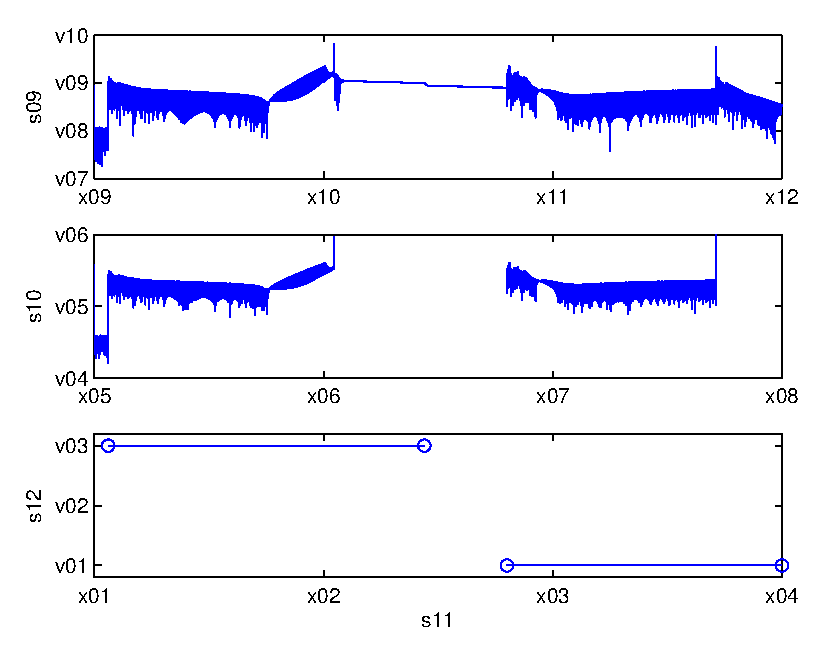
\includegraphics[width=15cm]{batt_noise_comp.eps}%
\end{psfrags}%
%
% End batt_noise_comp.tex
\end{document}
% See http://www.mathworks.de/matlabcentral/fileexchange/loadFile.do?objectId=4638
% for recent versions of laprint.m.
%
% created by:           LaPrint version 3.16 (13.9.2004)
% created on:           25-Feb-2014 20:15:36
% eps bounding box:     15 cm x 11.25 cm
% comment:              
%
\begin{psfrags}%
\psfragscanon%
%
% text strings:
\psfrag{s09}[b][b]{\color[rgb]{0,0,0}\setlength{\tabcolsep}{0pt}\begin{tabular}{c}$V_\text{cell}$ MSE [dBW]\end{tabular}}%
\psfrag{s10}[b][b]{\color[rgb]{0,0,0}\setlength{\tabcolsep}{0pt}\begin{tabular}{c}$i_\text{cell}$ MSE [dBW]\end{tabular}}%
\psfrag{s11}[t][t]{\color[rgb]{0,0,0}\setlength{\tabcolsep}{0pt}\begin{tabular}{c}Time (seconds)\end{tabular}}%
\psfrag{s12}[b][b]{\color[rgb]{0,0,0}\setlength{\tabcolsep}{0pt}\begin{tabular}{c}$R_L$\end{tabular}}%
%
% xticklabels:
\psfrag{x01}[t][t]{0}%
\psfrag{x02}[t][t]{5000}%
\psfrag{x03}[t][t]{10000}%
\psfrag{x04}[t][t]{15000}%
\psfrag{x05}[t][t]{0}%
\psfrag{x06}[t][t]{5000}%
\psfrag{x07}[t][t]{10000}%
\psfrag{x08}[t][t]{15000}%
\psfrag{x09}[t][t]{0}%
\psfrag{x10}[t][t]{5000}%
\psfrag{x11}[t][t]{10000}%
\psfrag{x12}[t][t]{15000}%
%
% yticklabels:
\psfrag{v01}[r][r]{-5}%
\psfrag{v02}[r][r]{0}%
\psfrag{v03}[r][r]{5}%
\psfrag{v04}[r][r]{-400}%
\psfrag{v05}[r][r]{-200}%
\psfrag{v06}[r][r]{0}%
\psfrag{v07}[r][r]{-300}%
\psfrag{v08}[r][r]{-200}%
\psfrag{v09}[r][r]{-100}%
\psfrag{v10}[r][r]{0}%
%
% Figure:
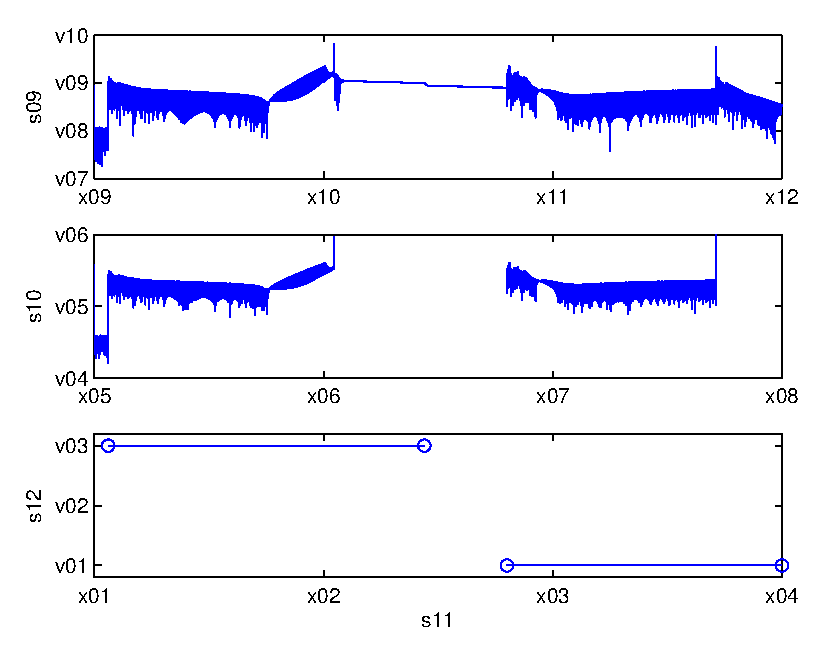
\includegraphics[width=15cm]{batt_noise_comp.eps}%
\end{psfrags}%
%
% End batt_noise_comp.tex
\end{document}
% See http://www.mathworks.de/matlabcentral/fileexchange/loadFile.do?objectId=4638
% for recent versions of laprint.m.
%
% created by:           LaPrint version 3.16 (13.9.2004)
% created on:           25-Feb-2014 20:15:36
% eps bounding box:     15 cm x 11.25 cm
% comment:              
%
\begin{psfrags}%
\psfragscanon%
%
% text strings:
\psfrag{s09}[b][b]{\color[rgb]{0,0,0}\setlength{\tabcolsep}{0pt}\begin{tabular}{c}$V_\text{cell}$ MSE [dBW]\end{tabular}}%
\psfrag{s10}[b][b]{\color[rgb]{0,0,0}\setlength{\tabcolsep}{0pt}\begin{tabular}{c}$i_\text{cell}$ MSE [dBW]\end{tabular}}%
\psfrag{s11}[t][t]{\color[rgb]{0,0,0}\setlength{\tabcolsep}{0pt}\begin{tabular}{c}Time (seconds)\end{tabular}}%
\psfrag{s12}[b][b]{\color[rgb]{0,0,0}\setlength{\tabcolsep}{0pt}\begin{tabular}{c}$R_L$\end{tabular}}%
%
% xticklabels:
\psfrag{x01}[t][t]{0}%
\psfrag{x02}[t][t]{5000}%
\psfrag{x03}[t][t]{10000}%
\psfrag{x04}[t][t]{15000}%
\psfrag{x05}[t][t]{0}%
\psfrag{x06}[t][t]{5000}%
\psfrag{x07}[t][t]{10000}%
\psfrag{x08}[t][t]{15000}%
\psfrag{x09}[t][t]{0}%
\psfrag{x10}[t][t]{5000}%
\psfrag{x11}[t][t]{10000}%
\psfrag{x12}[t][t]{15000}%
%
% yticklabels:
\psfrag{v01}[r][r]{-5}%
\psfrag{v02}[r][r]{0}%
\psfrag{v03}[r][r]{5}%
\psfrag{v04}[r][r]{-400}%
\psfrag{v05}[r][r]{-200}%
\psfrag{v06}[r][r]{0}%
\psfrag{v07}[r][r]{-300}%
\psfrag{v08}[r][r]{-200}%
\psfrag{v09}[r][r]{-100}%
\psfrag{v10}[r][r]{0}%
%
% Figure:
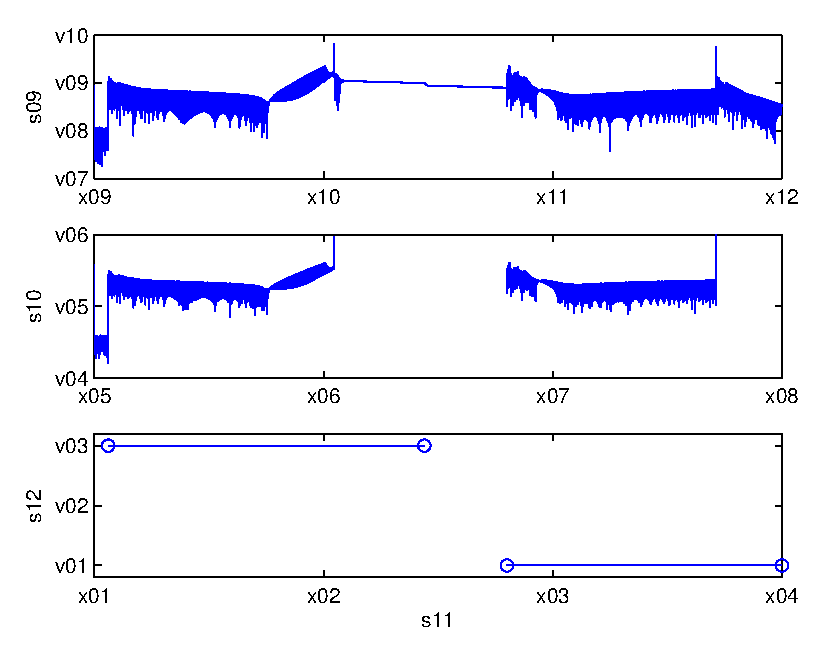
\includegraphics[width=15cm]{batt_noise_comp.eps}%
\end{psfrags}%
%
% End batt_noise_comp.tex
\end{document}
% See http://www.mathworks.de/matlabcentral/fileexchange/loadFile.do?objectId=4638
% for recent versions of laprint.m.
%
% created by:           LaPrint version 3.16 (13.9.2004)
% created on:           25-Feb-2014 20:15:36
% eps bounding box:     15 cm x 11.25 cm
% comment:              
%
\begin{psfrags}%
\psfragscanon%
%
% text strings:
\psfrag{s09}[b][b]{\color[rgb]{0,0,0}\setlength{\tabcolsep}{0pt}\begin{tabular}{c}$V_\text{cell}$ MSE [dBW]\end{tabular}}%
\psfrag{s10}[b][b]{\color[rgb]{0,0,0}\setlength{\tabcolsep}{0pt}\begin{tabular}{c}$i_\text{cell}$ MSE [dBW]\end{tabular}}%
\psfrag{s11}[t][t]{\color[rgb]{0,0,0}\setlength{\tabcolsep}{0pt}\begin{tabular}{c}Time (seconds)\end{tabular}}%
\psfrag{s12}[b][b]{\color[rgb]{0,0,0}\setlength{\tabcolsep}{0pt}\begin{tabular}{c}$R_L$\end{tabular}}%
%
% xticklabels:
\psfrag{x01}[t][t]{0}%
\psfrag{x02}[t][t]{5000}%
\psfrag{x03}[t][t]{10000}%
\psfrag{x04}[t][t]{15000}%
\psfrag{x05}[t][t]{0}%
\psfrag{x06}[t][t]{5000}%
\psfrag{x07}[t][t]{10000}%
\psfrag{x08}[t][t]{15000}%
\psfrag{x09}[t][t]{0}%
\psfrag{x10}[t][t]{5000}%
\psfrag{x11}[t][t]{10000}%
\psfrag{x12}[t][t]{15000}%
%
% yticklabels:
\psfrag{v01}[r][r]{-5}%
\psfrag{v02}[r][r]{0}%
\psfrag{v03}[r][r]{5}%
\psfrag{v04}[r][r]{-400}%
\psfrag{v05}[r][r]{-200}%
\psfrag{v06}[r][r]{0}%
\psfrag{v07}[r][r]{-300}%
\psfrag{v08}[r][r]{-200}%
\psfrag{v09}[r][r]{-100}%
\psfrag{v10}[r][r]{0}%
%
% Figure:
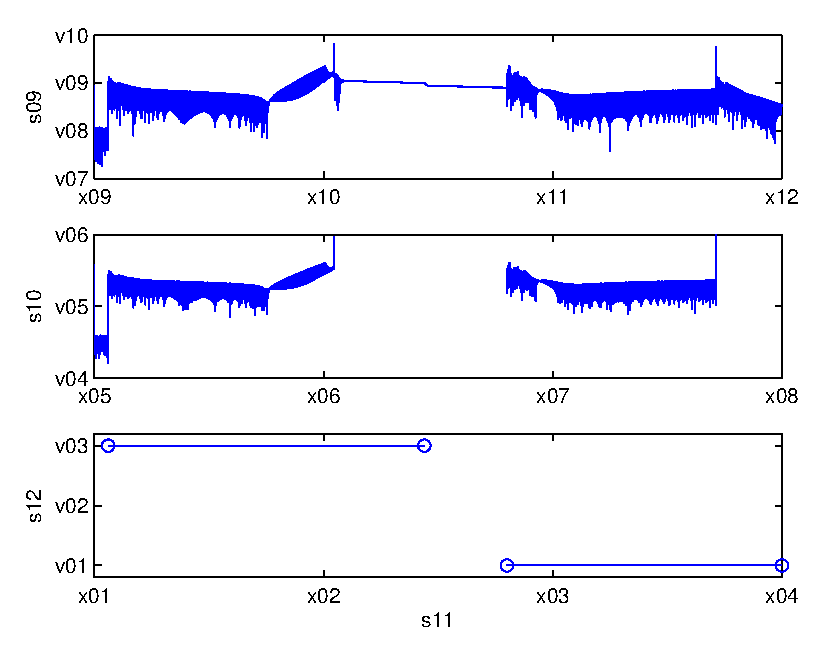
\includegraphics[width=15cm]{batt_noise_comp.eps}%
\end{psfrags}%
%
% End batt_noise_comp.tex
